\documentclass[11pt]{article}
\usepackage[preprint]{acl}
\usepackage{times}
\usepackage{latexsym}
\usepackage[T1]{fontenc}
\usepackage[utf8]{inputenc}
\usepackage{microtype}
\usepackage{graphicx}
\usepackage{booktabs}
\usepackage{amsmath,amssymb}
\title{Structural Primers for LLM Graph Reasoning:\\Reliability, Consistency, and Feature Resolution}
\author{Anonymous}
\begin{document}
\maketitle
\begin{abstract}
Can explicit structural summaries improve an LLM's use of a graph, beyond making individual answers easier to retrieve? We independently reanalyze 84,000 saved responses from GraphTalk, centered on 40-node graphs and Qwen3-1.7B/4B with and without native thinking. We reconstruct every graph and verify every target, evaluate exact answers under the recorded generation cap, and introduce a paired degree--neighborhood consistency diagnostic. Benefits are sharply task dependent: for plain 4B, a degree primer raises edge-count success from 2.00\% to 29.25\%, yet reduces joint correctness on local queries from 85.75\% to 76.50\%. Thinking-mode edge-count accuracy is strongly conditioned on completion. Additional density diagnostics expose majority-label effects in edge queries and a collapse in the diversity of rounded random-walk features. Structural information can help graph-query primitives, but neither summary availability nor internally consistent answers establishes general graph understanding or downstream graph-learning gains.
\end{abstract}

\section{Introduction}
Graph learning depends on retaining relations that a sequence representation can obscure. An LLM receiving an adjacency list must recover local neighborhoods, aggregate graph statistics, and preserve relations across its answers. A \emph{structural primer} supplies precomputed graph descriptors before the serialized graph. Such descriptors resemble the structural features used in graph neural networks, but textual availability does not guarantee effective use.

We ask: \textbf{When do structural primers improve reliable, mutually consistent graph answers, and how do topology and model mode limit those improvements?} This distinguishes three notions often conflated in graph reasoning: access to useful information, correct task execution within a budget, and agreement between related predictions. The distinction matters for graph ML pipelines that might use language models to inspect neighborhoods or compute structural features.

We conduct a fresh analysis of the saved GraphTalk experiments, rather than accepting prior aggregate reports. The core comparison uses Qwen3-1.7B and 4B in plain and native thinking modes on identical 40-node graphs. Our contributions are a target-verified, paired evaluation of seven prompt conditions; an output-level consistency probe linking degree and neighborhood predictions; and topology diagnostics separating feature precision and label imbalance from apparent reasoning gains. These are graph-query tasks, not trained node classification or held-out link prediction. Implications for those downstream settings are hypotheses, not measured transfer.

\section{Related Work}
\paragraph{Graphs as language.}
\citet{fatemi2024talk} show that graph serialization and prompting affect LLM graph reasoning. NLGraph tests multiple graph algorithms and finds limitations in solving graph problems from text \citep{wang2023nlgraph}. These motivate controlled graph-query evaluation, but an aggregate task score cannot establish whether two answers obey the same graph identity. NLGift studies generalization of graph reasoning across changes in settings and structures \citep{zhang2024nlgift}; our narrower, fixed-size analysis instead isolates response reliability and cross-query agreement within matched instances.

\paragraph{Structural features and interfaces.}
Random-walk structural encodings support graph representation learning \citep{dwivedi2022lspe}. GraphToken learns a graph encoder to condition an LLM \citep{perozzi2024graphtoken}, whereas GraphTalk supplies deterministic descriptors as text without training. This difference is substantive: a rounded textual feature may discard distinctions available to a numerical encoder. We measure that loss directly, without assuming that preserving every distinction improves language-model predictions.

\paragraph{Context and reasoning modes.}
Long-context studies document sensitivity to information position and input length \citep{liu2024lost,levy2024same}; irrelevant context can also disrupt reasoning \citep{shi2023distracted}. These motivate a filler comparison, but do not identify the cause of any GraphTalk effect. Qwen3 supports thinking and non-thinking modes \citep{yang2025qwen3}. We compare recorded outcomes under their actual caps, rather than treating accuracy among completed answers as unconditional reliability. Our contribution is an audited intersection of these concerns, not a claim to a new graph encoder or training method.

\section{Experimental Design}
\subsection{Graphs, tasks, and conditions}
The main dataset contains 100 independently seeded undirected Erd\H{o}s--R\'enyi graphs $G(40,p)$ at each $p\in\{.10,.20,.35,.50\}$. The same 400 graphs are reused across four model arms, six tasks, and seven conditions: 67,200 responses. A supplementary sweep adds $p\in\{.65,.75,.85\}$ for degree and edge-existence queries only (16,800 responses). It is not a six-task dense-graph replication.

Tasks ask for node count, edge count, one node's degree, its neighboring nodes, existence of one specified edge, or existence of a cycle. Node labels are integers 0--39. Degree and neighborhood queries share the same target node, enabling a paired consistency test. Every main graph has 40 nodes and a cycle; these two constant-label tasks are retained in the release but excluded from the main comparative table. Their success cannot distinguish structural reasoning from a constant answer.

Each zero-shot prompt contains a primer, the same incident adjacency-list encoding, and a question. \textbf{None} omits the primer. \textbf{Degree} lists all node degrees; \textbf{clustering} lists local clustering coefficients; \textbf{RWSE} gives $(P^2_{vv},P^3_{vv})$ per node, where $P=D^{-1}A$ and isolated rows are zero. Clustering and RWSE values are printed to two decimals. \textbf{Components} gives the number of connected components, not node memberships. \textbf{All} combines degree, clustering, and RWSE, excluding components. \textbf{Filler} enumerates the 40 nodes in generic sentences. It is an approximate verbosity control, not token matched across primers or devoid of graph information.

\subsection{Provenance and scoring}
We analyze repository snapshot \texttt{4b45c2435abe}, with file hashes and per-response provenance in the reproduction package. There are 84,002 raw records; two identical duplicates are removed, yielding 84,000 unique responses and 840 cells of 100. Independent graph reconstruction verifies every saved gold answer. No model is rerun or fine-tuned. Runner code specifies greedy generation and a native chat-template thinking switch; recorded capped outputs have 8,192 new tokens in the main sweep. Dense-extension caps are 2,048 for plain arms and 8,192 for thinking arms.

For graph $i$, condition $c$, and task $t$, our primary outcome is
\begin{equation}
 S_{ict}=\mathbf{1}[\hat y_{ict}=y_{it}]\,\mathbf{1}[\text{not capped}].
\end{equation}
Neighborhood equality is exact set equality; invalid or unparsed answers fail. This measures correct completion under the saved budget, rather than accuracy on a selected subset. We reuse the repository answer extractor for comparability and audit its behavior separately (Appendix~\ref{app:parser}); the extractor is not error-free.

Effects are paired differences on the same 400 graphs. We report density-stratified paired bootstrap 95\% intervals (4,000 resamples). Exact McNemar tests \citep{mcnemar1947} use binary outcomes; Benjamini--Hochberg adjustment \citep{benjamini1995} covers six primer contrasts within each arm/task/control family. These are exploratory families, not experiment-wide error control. We do not treat repeated tasks on the same graph as independent samples.

\subsection{Cross-query structural consistency}
Let $\hat d_i$ and $\hat N_i$ be extracted degree and neighborhood predictions for the same target in separate prompts. Define $C_i=1$ when both responses complete, the degree parses as an integer, neighborhood identifiers lie in 0--39, and $\hat d_i=|\hat N_i|$. Let $J_i=S_{i,\mathrm{degree}}S_{i,\mathrm{neighbors}}$ denote joint correctness. Since $J_i\leq C_i$, $C-J$ measures \emph{consistent but wrong} pairs. This tests a necessary graph identity at the output level; it does not measure a shared latent graph representation. We use the same paired inference, adjusting six contrasts separately for each arm and diagnostic.

\begin{table*}[t]
\centering\small
\begin{tabular}{llrrrrrrr}
\toprule
Arm & Task & None & Filler & Comp. & Clust. & RWSE & Degree & All \\
\midrule
1.7B & Degree & 60.50 & $-0.50$ & $+1.75$ & $+3.00$ & $+4.00$ & $+7.50^{*}$ & $+10.25^{*}$ \\
 & Neighbors & 72.50 & $-6.25^{*}$ & $+0.75$ & $+1.25$ & $+1.00$ & $+3.50$ & $+2.00$ \\
 & Edge exists & 70.50 & $-15.75^{*}$ & $-8.25^{*}$ & $+3.75$ & $+5.00$ & $+4.00$ & $+11.50^{*}$ \\
 & Edge count & 1.25 & $-0.50$ & $-1.00$ & $-0.50$ & $-0.75$ & $+3.00$ & $+0.75$ \\
\addlinespace[2pt]
1.7B-T & Degree & 76.25 & $-3.00$ & $-1.00$ & $+1.50$ & $+2.50$ & $+8.75^{*}$ & $+12.25^{*}$ \\
 & Neighbors & 78.75 & $+2.50$ & $+2.50$ & $+2.00$ & $+0.25$ & $+6.25^{*}$ & $+6.25^{*}$ \\
 & Edge exists & 99.00 & $-0.50$ & $-0.75$ & $-1.00$ & $-1.25$ & $-2.50$ & $-1.75$ \\
 & Edge count & 15.75 & $-1.50$ & $-0.75$ & $-1.25$ & $-3.25$ & $-3.25$ & $+5.00$ \\
\addlinespace[2pt]
4B & Degree & 99.25 & $-0.50$ & $+0.25$ & $-0.50$ & $-2.25^{*}$ & $-6.50^{*}$ & $-8.00^{*}$ \\
 & Neighbors & 86.00 & $-12.50^{*}$ & $+9.25^{*}$ & $+1.00$ & $+0.00$ & $-3.00$ & $-2.75$ \\
 & Edge exists & 90.50 & $-7.00^{*}$ & $-2.75$ & $+4.00^{*}$ & $-10.00^{*}$ & $-4.75^{*}$ & $-10.00^{*}$ \\
 & Edge count & 2.00 & $+1.25$ & $-1.25$ & $-1.25$ & $-1.50$ & $+27.25^{*}$ & $+3.75^{*}$ \\
\addlinespace[2pt]
4B-T & Degree & 97.00 & $+2.00$ & $+0.25$ & $+1.75$ & $-1.25$ & $+2.50$ & $+0.50$ \\
 & Neighbors & 95.50 & $+1.25$ & $+0.50$ & $-0.75$ & $+0.50$ & $+0.50$ & $-1.25$ \\
 & Edge exists & 99.75 & $+0.00$ & $-0.50$ & $-0.75$ & $-1.25$ & $+0.00$ & $-1.00$ \\
 & Edge count & 20.00 & $+12.25^{*}$ & $+24.75^{*}$ & $+24.75^{*}$ & $+10.25^{*}$ & $+8.50^{*}$ & $+1.75$ \\
\bottomrule
\end{tabular}
\caption{Main 40-node sweep: no-primer success (\%) and changes in percentage points for each primer, pooled equally across four densities ($n=400$ per cell). T denotes native thinking. Success requires an exact, uncapped answer. $^*$: paired McNemar BH-adjusted $q<.05$ within the six comparisons for that arm/task. Comp. is component count; Clust. is local clustering. Negative effects are retained. Full intervals and cell counts accompany the paper.}
\label{tab:main}
\end{table*}

\section{Results}
\subsection{Useful information is task specific}
Table~\ref{tab:main} shows no uniformly helpful primer. Degree supplies the answer to a degree query and a sufficient statistic for edge count through $|E|=\tfrac12\sum_v d_v$. Yet the strongest plain-4B gain is on edge count: 2.00\% to 29.25\%, a paired increase of 27.25 points (95\% CI [22.75,31.75]; 114 errors fixed, five introduced). Its degree-query success instead falls from 99.25\% to 92.75\%. For plain 1.7B, degree improves edge count by only 3.00 points, which does not survive the stated correction ($q=.101$); the 1.7B thinking effect is $-3.25$ points. Direct answer availability is therefore insufficient for dependable extraction or aggregation.

Clustering and component count produce the highest 4B-thinking edge-count success, both 44.75\%, versus 20.00\% without a primer. Each also exceeds filler (32.25\%) by 12.50 points, with paired intervals [7.50,17.75] and [6.75,18.01], respectively. These descriptors do not directly specify edge count. Moreover, every graph at $p\geq.20$ is connected: component count is constant over three main density strata. Its benefit cannot be explained solely by additional between-graph information in those strata. For $p=.20/.35/.50$, where component count is always one, component-primer success is 64/35/8\% versus filler's 46/22/1\%; the advantage persists without between-graph variation in that feature. Prompt framing, response trajectory, or other interactions remain possible explanations; the saved comparison does not separate them.

Combining features also fails to dominate. For 4B thinking, All reaches only 21.75\% edge-count success, below the 44.75\% of clustering alone. Conversely, All improves plain-1.7B edge existence by 11.50 points and degree by 10.25 points. Selecting a primer requires the model arm and task, not just the descriptor's mathematical relevance.

\subsection{Thinking accuracy depends on completion}
\begin{table}[t]
\centering\small
\begin{tabular}{lrrr}
\toprule
Arm & Completion & Conditional & Success \\
\midrule
1.7B & 70.25 & 1.78 & 1.25 \\
1.7B-T & 18.25 & 86.30 & 15.75 \\
4B & 100.00 & 2.00 & 2.00 \\
4B-T & 20.50 & 97.56 & 20.00 \\
\bottomrule
\end{tabular}
\caption{No-primer edge counting ($n=400$). Completion, accuracy conditional on completion, and unconditional success (all \%). Their product, after converting to proportions, gives success.}
\label{tab:completion}
\end{table}
Table~\ref{tab:completion} separates answer quality from completion. Among uncapped 4B-thinking edge-count responses, 97.56\% are correct; only 20.50\% complete, giving 20.00\% success. Thinking still improves over plain 4B's 2.00\%, but the conditional number substantially overstates reliability for an arbitrary graph. Similarly, 1.7B thinking achieves 86.30\% conditional accuracy but 15.75\% success.

Primer effects combine changes in completion and correctness. For 4B thinking, component count raises completion from 20.50\% to 45.50\% and success from 20.00\% to 44.75\%. Degree also raises completion, to 41.25\% versus baseline, but reaches only 28.50\% success. These are outcomes under a finite recorded cap, not evidence that unfinished reasoning could never produce a correct answer. Comparisons under longer or equal-compute budgets require new runs.

\subsection{Agreement is weaker than correctness}
\begin{table}[t]
\centering\small
\begin{tabular}{lrrr}
\toprule
Arm & None & Degree & All \\
\midrule
1.7B & 62.3/54.0 & 73.0/62.5 & 68.0/61.8 \\
1.7B-T & 81.0/71.0 & 81.0/76.5 & 83.5/79.5 \\
4B & 87.0/85.8 & 81.0/76.5 & 80.0/77.5 \\
4B-T & 94.0/93.8 & 96.0/95.8 & 93.8/93.2 \\
\bottomrule
\end{tabular}
\caption{Degree--neighborhood consistency/joint correctness ($C/J$, \%; 400 paired queries per cell). Agreement alone can mask jointly incorrect answers.}
\label{tab:joint}
\end{table}
For plain 1.7B, degree raises consistency to 73.00\%, but joint correctness is 62.50\%: 10.50\% of pairs satisfy the degree--cardinality identity while at least one answer is wrong (Table~\ref{tab:joint}). Relative to no primer, joint correctness improves by 8.50 points [4.25,12.75]. Thus useful improvement and residual structural errors coexist.

Plain 4B exposes a stronger trade-off. Degree helps global counting but decreases joint local correctness by 9.25 points [\,$-13.75,-4.75$\,], from 85.75\% to 76.50\% (28 pairs fixed, 65 broken). Component count instead raises it to 95.00\%, a 9.25-point gain [6.00,12.75]. Both contrasts survive correction and are unchanged by our targeted extraction sensitivity. In 4B thinking, baseline joint correctness is already 93.75\%; degree adds 2.00 points with interval [$-1.25$,5.00], providing no clear improvement. Better individual-task results should therefore not be assumed to yield uniformly better graph-query interfaces.

\begin{figure*}[t]
\centering
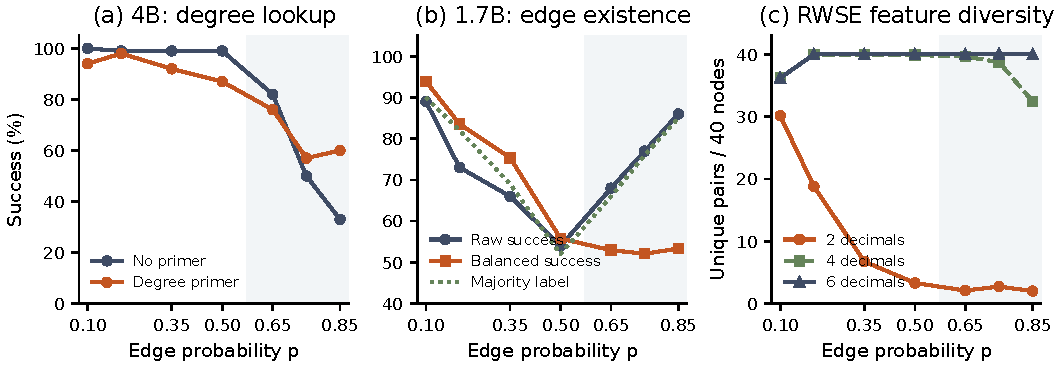
\includegraphics[width=\textwidth]{assets/density_diagnostics.pdf}
\caption{Density diagnostics on the same reconstructed graphs. Shading marks the supplementary sweep. (a) Degree information harms plain-4B degree lookup at several main densities but helps at $p=.85$. (b) Plain-1.7B no-primer edge success recovers at high density while balanced success remains near 50\%; majority label is a per-stratum constant predictor. (c) Mean distinct RWSE pairs among 40 nodes at alternative printing precisions. Only two-decimal features were given to models; four/six-decimal curves are feature analyses, not new LLM results. Each point uses 100 graphs; panels show descriptive means.}
\label{fig:density}
\end{figure*}

\subsection{Topology changes the interpretation}
The dense extension qualifies conclusions from the main sweep (Figure~\ref{fig:density}a). At $p=.50$, plain-4B degree success is 99\% without a primer and 87\% with degree information; at $p=.85$, it is 33\% and 60\%, respectively. Density increases adjacency-list size and neighborhood cardinality; the plain-arm output cap also changes from 8,192 to 2,048 in the extension. These data demonstrate effect heterogeneity across the recorded settings, but cannot isolate topology from input length or the changed cap, nor support a universal density threshold.

\paragraph{Label imbalance can hide failure.}
For plain 1.7B without a primer, edge-existence success rises from 54\% at $p=.50$ to 86\% at $.85$. However, the model answers Yes on 94\% and 99\% of queries, respectively. Balanced success, the mean of positive- and negative-class success, is only 55.77\% and 53.33\%. At $.85$, 85 of 100 queried edges exist, so an always-Yes rule already scores 85\%. The apparent recovery mostly tracks prevalence, not reliable rejection of absent edges. The small negative class (15 examples at $.85$) also limits precision.

\paragraph{Feature precision erases distinctions.}
The mean number of distinct two-decimal RWSE pairs per graph falls from 30.14 at $p=.10$ to 3.30 at $.50$ and 2.00 at $.85$ (Figure~\ref{fig:density}c). At $.50$, the most common pair covers 62.68\% of vertices on average. Reprinting reconstructed values at six decimals preserves 40.00 distinct pairs on average at $.50$ and 39.99 at $.85$. This is a quantifiable interface loss, not an absence of structural variation in the graph. It neither proves that node discrimination is required for these tasks nor causally explains the mixed RWSE effects in Table~\ref{tab:main}; no higher-precision LLM condition was run.

\section{Implications and Limitations}
For graph ML, the findings favor evaluating a proposed language interface at three levels: whether its features retain useful structural distinctions, whether each query completes correctly, and whether related outputs remain correct together. A degree list can provide an algorithmic shortcut without supporting more reliable local answers. Component-count effects show why a structural-sounding prompt should not automatically be credited with transmitting useful graph-specific information. Class-balanced evaluation is essential when changing graph density also changes answer prevalence.

The evidence is limited to small synthetic ER graphs, one serialization and label order, two model sizes, and saved deterministic generations. It does not test permutation invariance, real graph families, conventional predictive graph ML tasks, or learned representations. Density and prompt length co-vary; primers differ in length and answer content. Tests are exploratory, and intervals quantify graph-sample variation rather than model-training uncertainty. Extraction errors remain possible: the targeted audit changes consistency/joint-correctness cells by at most 1.25 points but is not exhaustive. Finally, capped exact responses count as failures by design; this is a completion-sensitive objective, not the only reasonable scoring policy.

A useful next experiment would cross feature precision with strictly matched prompt budgets, balance edge-query labels, and test unseen graph families and vertex permutations. Downstream feature construction or link prediction would then require separate held-out targets and leakage controls; degree primers in the present queries deliberately expose task-relevant answers.

\section{Conclusion}
On the central 40-node Qwen3 experiments, structural primers produce substantial but selective gains. Degree information improves plain-4B edge counting while damaging joint local correctness; thinking-mode gains must be interpreted alongside completion. Cross-query diagnostics, class balance, and feature-resolution checks reveal limitations hidden by individual accuracy. The supported conclusion is conditional utility for graph-query primitives, not general improvement in graph understanding or demonstrated transfer to downstream graph learning.
\label{mainend}
\bibliography{references}
\clearpage
\appendix
\section{Reproducibility and Data Integrity}
The analysis uses \url{https://github.com/GalBrk/GraphTalk} at source-data commit \texttt{4b45c2435abe} (full hash in the manifest). It reads 172 JSONL files matching the four arm names and \texttt{densfull40[hi].shard*.jsonl}. The manifest records file SHA-256 hashes. Every response retains its source filename and line number. The two duplicate records are identical under sorted JSON serialization; conflicting duplicates would cause the script to fail. Each unique arm/task/condition/density cell contains exactly 100 responses.

For density $p$ and graph index $i\in\{0,\ldots,99\}$, the graph seed is
\begin{align*}
 s={}&20260906+10^6(1+\operatorname{round}(1000p))\\
 &+40000+i.
\end{align*}
We reconstruct each edge by iterating over unordered vertex pairs in ascending order and comparing successive Python \texttt{random.Random(s)} draws to $p$. A separately initialized RNG selects the query vertex by \texttt{choice(range(40))}, or the queried endpoints by \texttt{sample(range(40),2)}. Degrees, components, cycle existence, neighborhoods, and edge counts are recomputed independently of the repository dataset generator. All saved golds agree semantically, including Boolean golds containing explanatory text. A cycle exists when $m>n-k$ for $k$ connected components.

The new \texttt{analyze.py} produces raw-derived response scores, topology descriptors, all density cells, paired intervals/tests, cross-query scores, extraction differences, observed caps, and the manifest. \texttt{reviewer\_audit.py} reproduces the audit samples and narrow correction sensitivity. \texttt{make\_assets.py} generates every empirical table and figure in the main paper from those outputs. The README specifies dependency versions, execution commands, and compilation. No inherited result table or significance output is used as an input to the analysis.

\section{Extraction Audit}\label{app:parser}
The primary extractor receives the full saved response. As a sensitivity, we apply it only to text after the final \texttt{</think>} marker. Predictions differ in 218 records, of which 11 are uncapped, changing 11 completion-sensitive outcomes. Manual inspection of all 11 uncapped cases shows that stripping is not uniformly corrective: four node-count answers improve, but four degree answers and one cycle answer become misparsed; another edge response uses an unsupported numeric Boolean, and a neighborhood response leaves its final answer blank after reasoning. We therefore retain the original parser instead of presenting the alternate parser as validated ground truth.

An independent reviewer additionally inspected one uncapped neighborhood response from each of 28 arm/condition cells, sampled with seed 472. One clear error triggered a targeted audit of all 24 uncapped singleton extractions with multi-node golds. Of these, 23 are extraction errors and 16 conceal correct final lists. Correcting only those manually inspected lists changes $C$ and $J$ by at most 1.25 percentage points per arm/condition (1.7B thinking with RWSE). All plain-4B cells and all $C-J$ cells are unchanged. The samples, raw response text, inspected corrections, and sensitivity table are released. This is a targeted robustness check, not an exhaustive validation or a confidence bound on total parser error.

\section{Additional Design Details}
Local clustering is $2T_v/[d_v(d_v-1)]$, set to zero when $d_v<2$. RWSE uses diagonal entries of the second and third powers of the random-walk transition matrix. Before formatting to two decimals, the implementation rounds features to six decimals; our descriptor analysis reproduces this convention. Distinct pairs are counted within each graph, then averaged over 100 graphs per density. This is not a measure of graph isomorphism discrimination or a learned embedding's expressivity.

The filler lists every node in a generic sentence, so it also reveals node count. Degree and All explicitly contain the queried degree and sufficient information for total edge count. These are intentional information-supplying interventions, but they prevent interpreting success gains as acquisition of an unaided graph algorithm. Components is a single graph-level count, unlike the node-wise tables. Primer length is consequently confounded with content.

Main-sweep mean edge counts are 78.64, 155.12, 272.98, and 389.40 at $p=.10,.20,.35,.50$. The fraction connected is .48 at $.10$ and 1.00 at every higher sampled density. All 700 reconstructed graphs contain cycles. The dense extension evaluates only degree and edge existence. Main-sweep task results use 400 graphs per cell regardless of parsing or completion; no completed-only filtering enters Table~\ref{tab:main}.

Bootstrap differences resample graph-level paired outcomes independently within each density and combine the four strata equally. The fixed bootstrap seed is 1947. Tests use discordant correct/incorrect pairs, never fractional neighborhood F1. F1 is retained in output files as a secondary descriptive score. The six contrasts against filler form separate adjustment families from the six contrasts against None. Cross-query families separately adjust consistency, joint correctness, and consistent-but-wrong outcomes. All reported comparisons remain exploratory; selected intervals are not simultaneous confidence intervals.
\end{document}
